% Kapitel 3 mit den entsprechenden Unterkapiteln
% Die Unterkapitel können auch in separaten Dateien stehen,
% die dann mit dem \include-Befehl eingebunden werden.
%-------------------------------------------------------------------------------
\chapter{Implementierungsentwurf}
%Dieser Abschnitt hat die Aufgabe, alle verwendeten Klassen und Bibliotheken zu
%dokumentieren. Dabei wird jede Komponente aus dem Grobentwurf gesondert
%betrachtet. F\"ur Entwurfsentscheidungen, die mehr als eine Komponente betreffen,
%wird mit Verweisen zwischen den Dokumentationen der Komponente gearbeitet.  Es
%sind dabei so viele Unterabschnitte einzuf\"ugen, wie Komponenten vorhanden sind.


\section{Gesamtsystem}
%F\"ugen Sie hier bitte das Komponentendiagramm aus dem Grobentwurf ein und
%erl\"autern Sie kurz die Funktionen der Komponenten.
\begin{figure}[!htb]
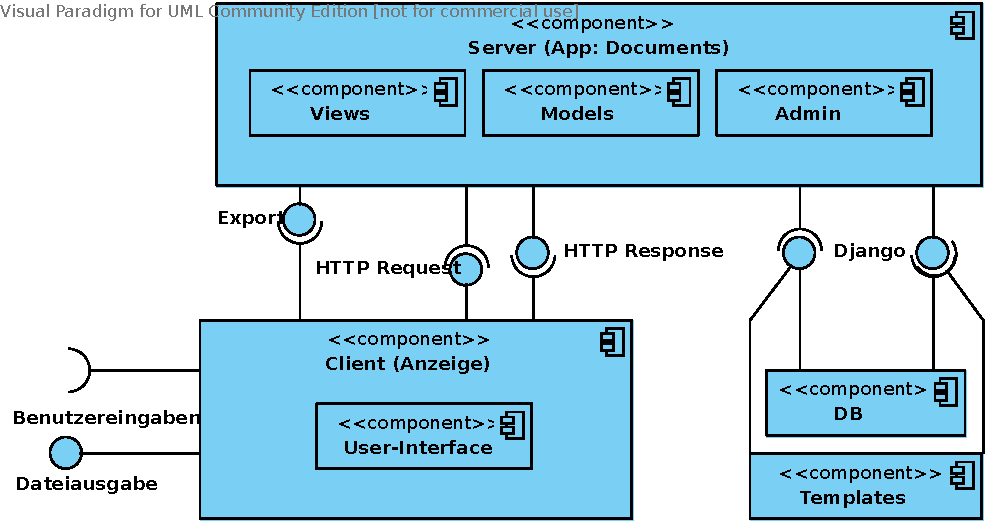
\includegraphics[width=0.8\linewidth]{bilder/Komponentendiagramm.pdf}
\caption{Komponentendiagramm}
\label{fig:KompDiagramm}
\end{figure}

Die Komponente Client fungiert als Schnittstelle zwischen Benutzer und der 
Applikation Documents. Sie nimmt Eingaben des Benutzers entgegen und bereitet 
HttpResponses des Servers auf.

Die Komponente Views prozessiert HttpRequests des Clients, leitet Aufrufe an die
jeweiligen Templates weiter und füllt diese mit geforderten Informationen.

Die Komponente Models bildet die Struktur der DB ab.

Die Komponente Admin stellt die gesamten Admin-Funktionen zur Verfügung, also 
Funktionen, welche nicht von normalen Benutzern durchgeführt werden sollen.

Die Komponente DB stellt die Datenbank der gesamten Applikation dar.
Sie liefert gewünschte Informationen, z.B. über Dokumente, Benutzer, deren 
ausgeliehenen Bücher etc.

Die Komponente Templates stellt die HTML-Seiten dar, welche durch andere 
Komponenten(Views,Admin...) mit Informationen befüllt werden.    



\section{Implementierung von Komponente
         1: Client}

%Beschreiben Sie hier bitte die Implementierung der Komponente. Erl\"autern Sie
%bitte dabei, welche Entwurfsmuster und Bibliotheken Sie verwenden. Die
%Implementierung wird dabei durch Klassendiagramme dokumentiert.

Der Client musste nicht im eigentlichen Sinne implementiert, sondern eher
integriert werden. Dazu wurden verschiedene Browser getestet und der
Programmcode bei auftretenden Fehlern angepasst. Die Integration dieser
Komponente ist wichtig, da das Systen später nicht nur von wenigen Browsern aus
funktionieren soll.
Der Client dient als Schnittstelle des Benutzers mit dem eigentlichen Programm
auf dem Server. Mittels eines Browsers, der von uns nicht festgelegt wird, werden
die Webseitencodes, die der Server an den Clienten auf dessen Anfragen sendet,
in die für den Benutzer verständliche Form einer Webseite gebracht.

\subsection{Paketdiagramm}
Hier die Abbildung \ref{fig:PDclient} : Das Paketdiagramm der Komponente Client.
\begin{figure}[H]
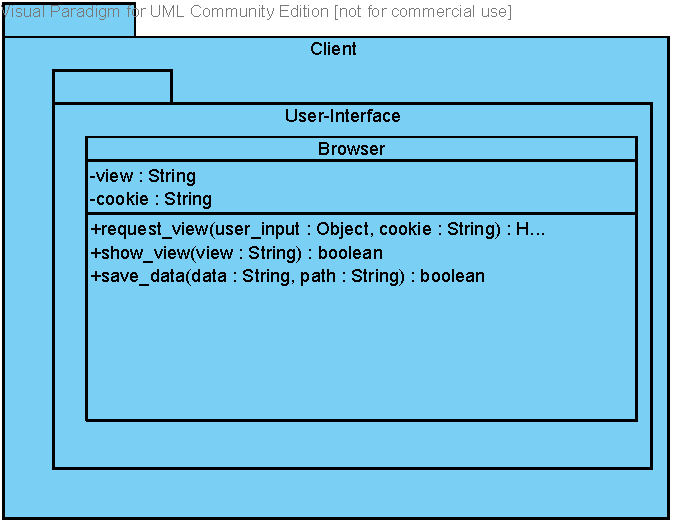
\includegraphics[width=0.8\linewidth]{bilder/Paketdiagramm_client.pdf}
\caption{Paketdiagramm Client}
\label{fig:PDclient}
\end{figure}
\subsection{Erl\"auterung}

Da als Client mehrere verschiedene Browser in Frage kommen, können die genauen
Funktionen dieser Komponente hier nicht beschrieben werden. Die für uns
wichtigen Funktionen sind die Möglichkeit eine Anfrage an unseren Server zu
stellen, einen Webseitencode darstellen zu können und eine Datei lokal zu
speichern. Dabei funktioniert die Kommunikation mit dem Server über
Http-Requests und Http-Responses. Für die Korrektheit der Ergebnisse mancher
Anfragen wird der lokale Cookie benötigt und deswegen mitgesendet. 
Auf eine Anfrage per HttpRequest kann der Browser entweder einen Webseitencode 
oder eine Datei als Http-Response erhalten. Je nachdem was er erhält, ruft er 
die passende Funktion auf. 

%Die verwendeten Attribute, Aufgaben und Kommunikationspartner sind f\"ur jede
%Klasse kurz zu erl\"autern. Die ankommenden Nachrichten beziehen sich dabei auf
%die Sequenzdiagramme der Feinanalyse im Grobentwurf und stellen meist
%aufzurufende Methoden der Klasse dar.  Reine get- / set-Methoden oder
%Bibliotheksfunktionen brauchen nicht aufgef\"uhrt zu werden.

\section{Implementierung von Komponente
         2: View}

%Beschreiben Sie hier bitte die Implementierung der Komponente. Erl\"autern Sie
%bitte dabei, welche Entwurfsmuster und Bibliotheken Sie verwenden. Die
%Implementierung wird dabei durch Klassendiagramme dokumentiert.

Die Views sind einer der essentiellen Bestandteile des Django-Frameworks. Sie
bestimmen die Art und Weise wie Templates aufgerufen werden, welche
Informationen die Templates bekommen und wie die Daten aus den Templates
verarbeitet werden. Sie sind die Schnittstelle zwischen den Templates und dem
Rest des Programmes.

\subsection{Paketdiagramm}
Hier die Abbildung \ref{fig:PDviews} : Das Paketdiagramm der Komponente Views.
\begin{figure}[H]
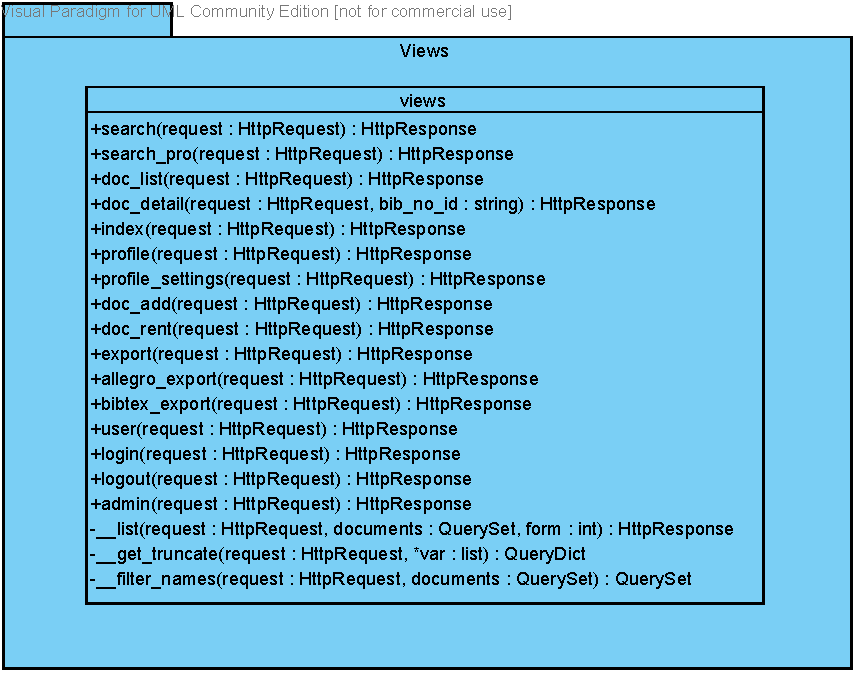
\includegraphics[width=0.8\linewidth]{bilder/Paketdiagramm_views.pdf}
\caption{Paketdiagramm Views}
\label{fig:PDviews}
\end{figure}
\subsection{Erl\"auterung}
Die Komponente View besteht aus einem einzigen Paket, welches für jede
beachbsichtigte Art des Aufrufs eines Templates eine Funktion zur Verfügung
stellt. Dabei erhalten die Funktionen über einen Http-Request Informationen, die
in der Funktion verarbeitet werden und geben einen Http-Response zurück, welche
den fertigen Webseitencode enthält. Da die Funktion doc\_detail
teilweise indirekt von anderen Funktionen der Komponente View aufgerufen wird,
benötigt sie noch den zusätzlichen Parameter, der ihr mitteilt, welches Dokument
dargestellt werden soll.


\section{Implementierung von Komponente
         3: Models}

%Beschreiben Sie hier bitte die Implementierung der Komponente. Erl\"autern Sie
%bitte dabei, welche Entwurfsmuster und Bibliotheken Sie verwenden. Die
%Implementierung wird dabei durch Klassendiagramme dokumentiert.

Die Komponente Models stellt die Struktur der Datenbank dar. Das
Django-Framework nimmt diese Struktur und setzt sie selbstständig in eine SQLite Datenbank
um. Jede Klasse dieser Komponente ist das Muster für eine Tabelle in der
Datenbank.

\subsection{Paketdiagramm}
Hier die Abbildung \ref{fig:PDmodels} : Das Paketdiagramm der Komponente Models.
\begin{figure}[H]
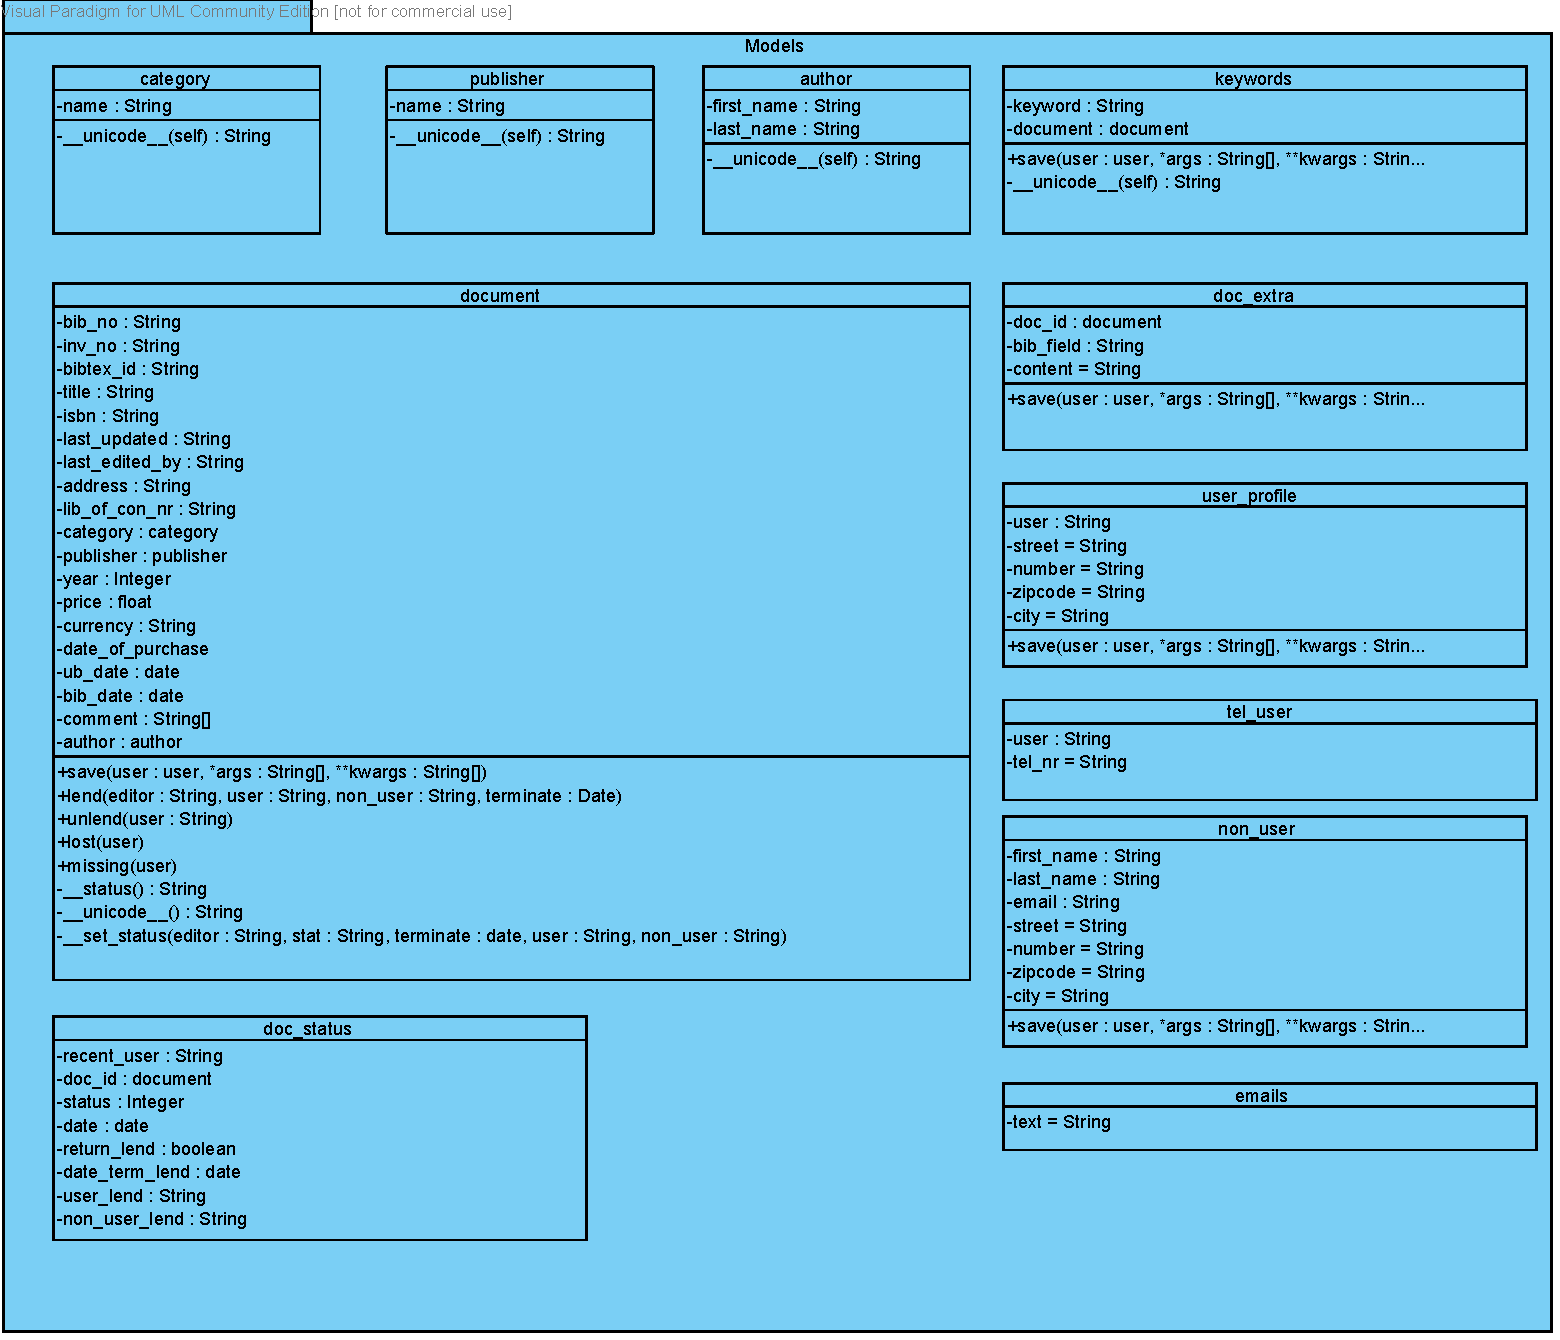
\includegraphics[width=0.9\linewidth]{bilder/Paketdiagramm_models.pdf}
\caption{Paketdiagramm Models}
\label{fig:PDmodels}
\end{figure}
\subsection{Erl\"auterung}
Jede Klasse stellt eine Tabelle in der Datenbank dar und jedes Attribut eine
Spalte dieser Tabelle. Wenn ein Attribut den Typ einer anderen Klasse aus den
Models besitzt, stellt dies eine Beziehung in der späteren Datenbank dar.
Mehrere Klassen haben die unicode-Funktion. Diese Funktion definiert, wie eine
Tabelle bzw. eine Zeile dieser Tabelle als String dargestellt werden soll.
Mehrere Klassen haben die save-Funktion, welche gerade durchgeführte Änderungen
unter Angabe des Editors sofort speichert. Die Klasse \lstinline{documents} hat außerdem
die Funktionen lost, missing, unlend und lend, welche den Status des jeweiligen
Dokumentes ändern können.

\section{Implementierung von Komponente
         4: Admin}

%Beschreiben Sie hier bitte die Implementierung der Komponente. Erl\"autern Sie
%bitte dabei, welche Entwurfsmuster und Bibliotheken Sie verwenden. Die
%Implementierung wird dabei durch Klassendiagramme dokumentiert.

Die Komponente Admin stellt die Funktionen zur Veränderung von Daten zur Verfügung,
die nicht von normalen Benutzern durchgeführt werden sollen.

\subsection{Paketdiagramm}
Hier die Abbildung \ref{fig:PDadmin} : Das Paketdiagramm der Komponente Admin.
\begin{figure}[H]
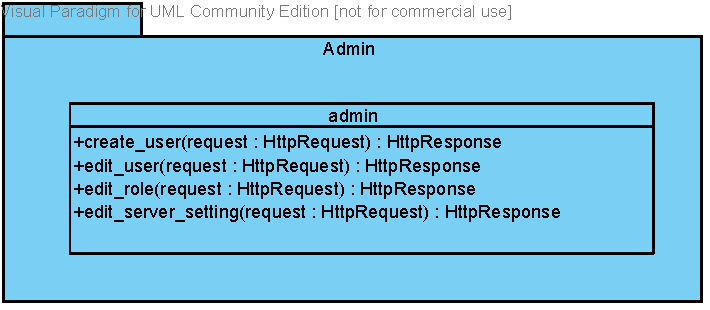
\includegraphics[width=0.8\linewidth]{bilder/Paketdiagramm_admin.pdf}
\caption{Paketdiagramm Admin}
\label{fig:PDadmin}
\end{figure}
\subsection{Erl\"auterung}
Die Eingabe der Daten für die Adminfunktionen funktioniert auch hier über
einen Http-Request. Die Http-Response besteht hier allerdings nur aus einer
Nachricht, dass die Änderung funktioniert hat und aus eventuell der Ansicht der
geänderten Daten. Es ist mit diesen Funktionen möglich, in der Datenbank neue
User zu erstellen und zu ändern, die verfügbaren Rollen zu bearbeiten und die
generellen Einstellungen des Servers zu ändern. 

\section{Implementierung von Komponente
         5: DB und Template}

%Beschreiben Sie hier bitte die Implementierung der Komponente. Erl\"autern Sie
%bitte dabei, welche Entwurfsmuster und Bibliotheken Sie verwenden. Die
%Implementierung wird dabei durch Klassendiagramme dokumentiert.

Die Komponente DB besteht aus einem Datenbanksystem. 
Dabei übernimmt das Django-Framework die komplette Kommunikation mithilfe 
der Komponente Models. 
Die Templates sind eine statische Komponente, auf die das Django-Framework
zugreift, sobald sie von der Komponente View benötigt werden. 

\subsection{Paketdiagramm}
Die Paketdiagramme wurden weggelassen. Siehe dazu den Punkt Erläuterung.

\subsection{Erl\"auterung}
Ein Paketdiagramm für das komplette Datenbanksystem wird nicht eingefügt, da es
sich um ein bestehendes System handelt. Genaueres zu der Struktur der
Datenbank wird in \ref{kap4} erläutert.
Auf ein Paketdiagramm für die Komponente Templates wird verzichtet, da diese
keinerlei Funktionen besitzt, sondern nur von anderen Komponenten mit Daten
gefüllt und weitergeleitet wird. Diese Kommunikation wird vom Django-Framework
durchgeführt, für das ein Paketdiagram ebenfalls die Maße dieses Dokumentes
sprengen würde.
